
\chapter{Package implementation in R}
\label{cha:R}

Once understood what is a Bitcoin Cash, how works the technology behind it and the
reasons why it was created. Its time to start and read some data from the blockchain
in order to put into practice what we have learned in the above chapters. Moreover,
after the data is imported, it is a good practice to analyze the data in such a way as to 
get useful information out of it. To do so, the R programming language will be used.

\section{R}
\label{sec:enivirionment}

R is an Open Source software for statistical computing(linear and nonlinear
 modeling, classical statistical tests, time-series analysis, classification,
 clustering) and graphics. One of R’s strengths is the ease with which well-designed 
 publication-quality plots can be produced, including mathematical symbols and 
 formulae where needed.\\
R is designed around a true computer language, and it allows users to add additional 
functionality by defining new functions. Much of the system is itself written in the 
R which makes it easy for users to follow the algorithmic choices made. But, for
computationally-intensive tasks, C, C++ and Fortran code can be linked and called 
at run time. Furthermore, thanks to its Open Source nature, it can be easily extended
via "Packages" even written by the user himself.\cite{r}

\section{Feasibility study}
\label{sec:study}

The goal for this project is to extend the R language with a package which allows us
to read and analyze the information into the Bitcoin Cash blockchain.\\
To make it in the best way, firstly, was done a research of the existing 
implementations, unfortunately, without any result. But, it brings us two 
completely different ways to realize the package. \\
The first one was to turn the used device into a node of the Bitcoin Cash network.
This leads the user to download all the blockchain and make all the queries locally.
As a result, the queries will be very fast and all the data of the blockchain can
be manipulated as you desire. But, on the other hand, storing all the blockchain 
requires a lot of space on your device (around 143 GigaByte on 13/9/2019). So making
a package of that size doesn't seem to be the best option.\\
For these reasons, the second way was chosen. Although it is the slowest implementation,
it avoids the need to become a node of the network, making the installation of the
package very simple and fast. That was obtained by relying on a service provider (SP).

\section{Package integration}
\label{sec:integration}

Once decided the more convenient option to adopt, it was necessary to do another
research phase. In fact, it is pretty difficult to find a SP which 
not only implemented an "Application Programming Interface" (API) where you can 
make queries an have the wanted data as a response. But also makes it public, 
so anyone can use it. Additionally, the service providers were chosen also 
according to the amount of data provided, the format of the response and the 
number of queries you are allowed to make. At the end, the picks were:
\begin{itemize}
    \item Blockdozer Explorer
    \item Blockchair
\end{itemize} 
The motivation for these two options is the fact that they are complementary.
The first one allows an unlimited number of queries returning essential information.
The second one instead, has a limit of 30 queries per minute but returns more 
and better-formatted data. 

Let's start with the technical implementation by saying that to maintain all the R project, 
was used the RStudio editor.\\ 
First of all, it is necessary to create and manage a new package in R. For this 
purpose, some other packages are required : 
\begin{itemize}
    \item "devetools"   - To manage the project and the source code of the new package.
    \item "roxygenize2" - To handle all the documentation of the package.
\end{itemize}
Then it is necessary to install the other two packages to handle the data and the connection with 
the service providers.
\begin{itemize}
    \item "httr"        - To perform correctly the Http requests to the service providers and receive the linked response
    \item "jsonlite"    - To manipulate and store the received data, in order to have a good dataset for the future analysis
\end{itemize}
Now we are ready to perform a simple query to an API. Let's say that we want to know
some information about a specific Bitcoin Cash address. After choosing the appropriate SP,
we have to read their documentation and see how to correctly build the Http request. 
In this case, the pattern is: \medskip

\textit{GET /api/addr/\{paymentAddress\}[?noTxList\&from\&to\&returnLegacyAddresses]}
\\
\begin{figure}[h]
    \centering
    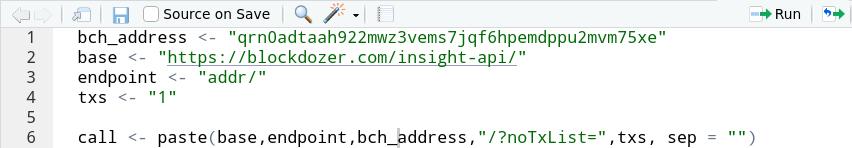
\includegraphics[height=2cm]{create_call.png}
    \caption{Example of the building of an Http request}
    \label{fig:request}
\end{figure}\\
With a few lines code, we can then construct a possible request for our information. 
As a result we can have:\medskip

\textit{https://blockdozer.com/insight-api/addr/qrn0adtaah922mwz3vems7jqf6hpemdppu2mvm75xe/?noTxList=1}
\medskip\\
As said before, the response will be in a json format and will be handled thanks to the
jsonlite package. But due to the multiple ways to manipulate the data, it is 
suggested to go on the GitHub repository\footnote{\url{github.com/PopBogdan97/bCashReader}} and take a look at the source code.
\begin{figure}[h]
    \centering
    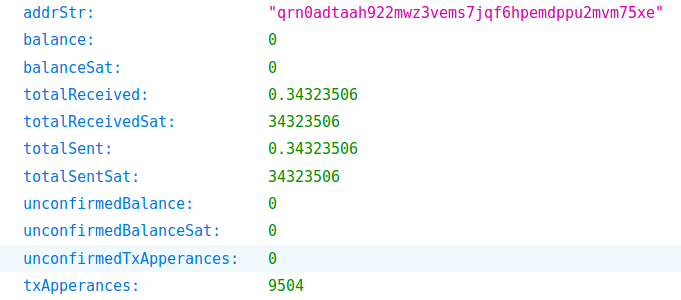
\includegraphics[height=5cm]{json_sample.png}
    \caption{Example json response}
    \label{fig:response}
\end{figure}\pagebreak


\subsection{Commands}
\label{sec:commands}

Due to the multiple data formats provided by the Service Providers and the 
different information that can be retrieved from the Bitcoin Cash blockchain, 
we can subdivide all the implemented commands in four macro categories.\medskip
\textbf{Address Commands}
\begin{table}[!ht]
    \centering
    \begin{tabular}{||l|p{6cm}||}
    \hline
    \textbf{Function}                          & \textbf{Description}                                                  \\ \hline
    addr\_balance(hash string)                 & Get the balance of a Bitcoin Cash address.                            \\ \hline
    addr\_history(hash string)                 & Get the general data (history) of a Bitcoin Cash address.             \\ \hline
    addr\_totalReceived(hash string)           & Get the total amount of Bitcoin Cash received by the address.         \\ \hline
    addr\_totalSent(hash string)               & Get the total amount of Bitcoin Cash sent by the address.             \\ \hline
    addr\_txApperances(hash string)            & Get the total amount of transactions made by the address.             \\ \hline
    addr\_txs(hash string)                     & Get the all the transactions made by the address.                     \\ \hline
    addr\_unconfirmedBalance(hash string)      & Get the unconfirmed balance of a Bitcoin Cash address.                \\ \hline
    addr\_unconfirmedTransactions(hash string) & Get the total amount of unconfirmed transactions made by the address. \\ \hline
    addr\_utxo(hash string)                    & Get the unspent transactions (UTXO) of an address.                    \\ \hline
    \end{tabular}
    \end{table}
\medskip 
\textbf{Block Commands}
\begin{table}[!ht]
    \centering
    \begin{tabular}{||l|p{6cm}||}
    \hline
    \textbf{Function}                          & \textbf{Description}                                                  \\ \hline
    block\_byDate("yyyy-MM-dd" string)                 & Get all the blocks in a specific Date with the format yyyy-MM-dd.                          \\ \hline
    block\_byDateCount("yyyy-MM-dd" string)    & Get the block count in a specific Date with the format yyyy-MM-dd.             \\ \hline
    block\_byHash(hash string)                 & Get the information of a specific Bitcoin Cash block (without the transactions).         \\ \hline
    block\_byHashRaw(hash string)              & Get the raw information of a specific Bitcoin Cash block.             \\ \hline
    block\_byHashTxs(hash string)              & Get the transaction hashes of a specific Bitcoin Cash block.             \\ \hline
    block\_byHeight(height integer)            & Get the informations contained in a specific Bitcoin Cash block.                     \\ \hline
    \end{tabular}
    \end{table}\pagebreak
\medskip 
\textbf{Transaction Commands}
\begin{table}[!ht]
    \centering
    \begin{tabular}{||l|p{6cm}||}
    \hline
    \textbf{Function}                          & \textbf{Description}                                                  \\ \hline
    txs\_byHash(hash string)                   & Get the all the information of a specific transaction\footnotemark[2].                          \\ \hline
    txs\_byHashIn(hash string)         & Get the all the information of a specific transaction inputs\footnotemark[2].      \\ \hline
    txs\_byHashOut(hash string)                & Get the all the information of a specific transaction outputs\footnotemark[2].          \\ \hline
    \end{tabular}
    \end{table}
\footnotetext[2]{To see the description of the values retrieved visit: \url{https://github.com/Blockchair/Blockchair.Support/blob/master/API_DOCUMENTATION_EN.md#link_chainstats} in Dashboard/transaction}
\medskip 
\textbf{Chain Commands}
\begin{table}[!ht]
    \centering
    \begin{tabular}{||p{6.2cm}|p{6cm}||}
    \hline
    \textbf{Function}                          & \textbf{Description}                                                  \\ \hline
    chain\_currency()                           & Get the Bitcoin Cash current value..                          \\ \hline
    chain\_stats()                              & Get the Bitcoin Cash current blockchain stats\footnotemark[3].              \\ \hline
   \end{tabular}
    \end{table}
\footnotetext[3]{To see the description of the values retrieved visit: \url{https://github.com/Blockchair/Blockchair.Support/blob/master/API_DOCUMENTATION_EN.md#link_chainstats"} in Dashboard/stats.}


\section{Usage samples}
\label{sec:sample}
repository